\usetikzlibrary{calc}

\definecolor{DarkPink}{rgb}{0.55, 0.05, 0.37}

\newcommand*{\GridSize}{3}

\newcommand*{\ColorCells}[1]{% #1 = list of x/y/color
  \foreach \x/\y/\color/\text in {#1} {
    \node [fill=\color, draw=black, thick ,minimum size=1cm, line width=.8pt] 
      at (\x-.5,\GridSize+0.5-\y) [text=white] {\text};
    }%
}%

\tikzset{near start abs/.style={xshift=1cm}}
%%%%%


%\listfiles
\scalebox{0.42}{ %%% scale it
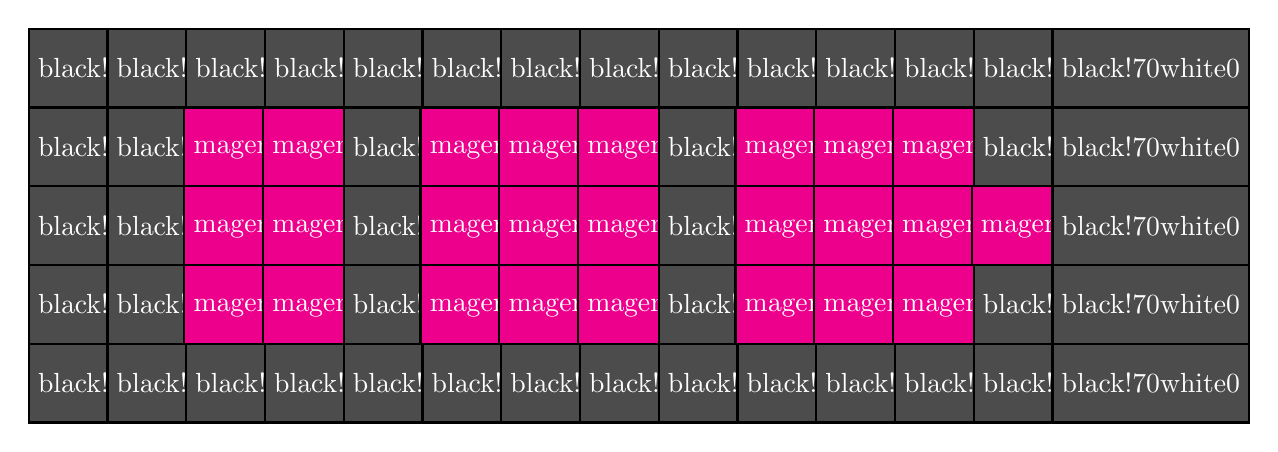
\begin{tikzpicture}
    \begin{scope}[thick,local bounding box=name]
    
         \ColorCells{
            1/1/black!70/0,
            2/1/black!70/0,
            3/1/black!70/0,
            4/1/black!70/0,
            5/1/black!70/0,
            6/1/black!70/0,
            7/1/black!70/0,
            8/1/black!70/0,
            9/1/black!70/0,
            10/1/black!70/0,
            11/1/black!70/0,
            12/1/black!70/0,
            13/1/black!70/0,
            14/1/black!70/0,
            1/2/black!70/0,
            2/2/black!70/0,
            3/2/magenta/1,
            4/2/magenta/1,
            5/2/black!70/0,
            6/2/magenta/1,
            7/2/magenta/1,
            8/2/magenta/1,
            9/2/black!70/0,
            10/2/magenta/1,
            11/2/magenta/1,
            12/2/magenta/1,
            13/2/black!70/0,
            14/2/black!70/0,
            1/3/black!70/0,
            2/3/black!70/0,
            3/3/magenta/1,
            4/3/magenta/1,
            5/3/black!70/0,
            6/3/magenta/1,
            7/3/magenta/1,
            8/3/magenta/1,
            9/3/black!70/0,
            10/3/magenta/1,
            11/3/magenta/1,
            12/3/magenta/1,
            13/3/magenta/1,
            14/3/black!70/0,
            1/4/black!70/0,
            2/4/black!70/0,
            3/4/magenta/1,
            4/4/magenta/1,
            5/4/black!70/0,
            6/4/magenta/1,
            7/4/magenta/1,
            8/4/magenta/1,
            9/4/black!70/0,
            10/4/magenta/1,
            11/4/magenta/1,
            12/4/magenta/1,
            13/4/black!70/0,
            14/4/black!70/0,
            1/5/black!70/0,
            2/5/black!70/0,
            3/5/black!70/0,
            4/5/black!70/0,
            5/5/black!70/0,
            6/5/black!70/0,
            7/5/black!70/0,
            8/5/black!70/0,
            9/5/black!70/0,
            10/5/black!70/0,
            11/5/black!70/0,
            12/5/black!70/0,
            13/5/black!70/0,
            14/5/black!70/0
         }

    \end{scope}
\end{tikzpicture}
} %%% case